\documentclass[ignorenonframetext,xcolor=pdflatex,table,dvipsnames,serif]{beamer}
%\usetheme[unit=biostat,footstyle=low]{Frederiksberg}
%\usetheme[sund]{Frederiksberg}
\usetheme[background = dark]{metropolis}

\usepackage[utf8]{inputenc}
\usepackage[english]{babel}
\usepackage{amssymb}
\usepackage{amsmath}
\usepackage{fancyvrb}
\usepackage{tikzsymbols}

\DeclareMathOperator{\E}{\mathbb{E}}
\DeclareMathOperator{\Var}{Var}
\DeclareMathOperator{\Erf}{Erf}
\DeclareMathOperator{\Cov}{Cov}
\DeclareMathOperator{\Multinomial}{Multinomial}
\DeclareMathOperator{\logit}{logit}
\DeclareMathOperator*{\argsup}{arg\,sup}
\newcommand\independent{\protect\mathpalette{\protect\independenT}{\perp}}
\def\independenT#1#2{\mathrel{\rlap{$#1#2$}\mkern2mu{#1#2}}}

\title{The Trendiness of Trends}
%\date{\today}
\date{April 9\textsuperscript{th} 2019, DSTS meeting}
\author{Andreas Kryger Jensen \scriptsize (joint with Claus Ekstrøm)}
\institute{Biostatistics, Institute of Public Health\\ University of Copenhagen}



\begin{document}

\frame[plain]{\titlepage}
 
%\begin{frame}{Roadmap}
%  \setbeamertemplate{section in toc}[sections numbered]
%  \tableofcontents[hideallsubsections]
%\end{frame}
 
%\maketitle

\section{The problem}

\begin{frame}{Changes in trends}
A statement often seen in the news is that at \alert{this very moment} we see a significant change in the trend of something.

\vspace{0.5cm}

\begin{center}
,,The trend has broken''
\end{center}

\vspace{0.5cm}

Recent examples from the Danish public news:
\begin{itemize}
  \item{Proportion of injuries from fireworks on New Year's Eve}
  \item{Proportion of children being baptized}
  \item{Average price of a one-family house}
  \item{\underline{Proportion of smokers}}
\end{itemize}
\end{frame}

\begin{frame}{Fundamental questions}
It is \alert{trendy} to talk about changes in \alert{trends}.

But...
\begin{itemize}
  \item{What is a \alert{trend}?}
  \item{What is a change in a \alert{trend}?}
  \item{What is the ,,\alert{trendiness}'' of a \alert{trend}?}
  \item{How many times has the \alert{trend} changed?}
\end{itemize}
Can we quantify and estimate answers to these questions?
\end{frame}

\begin{frame}{Politiken, January 02, 2019}
\center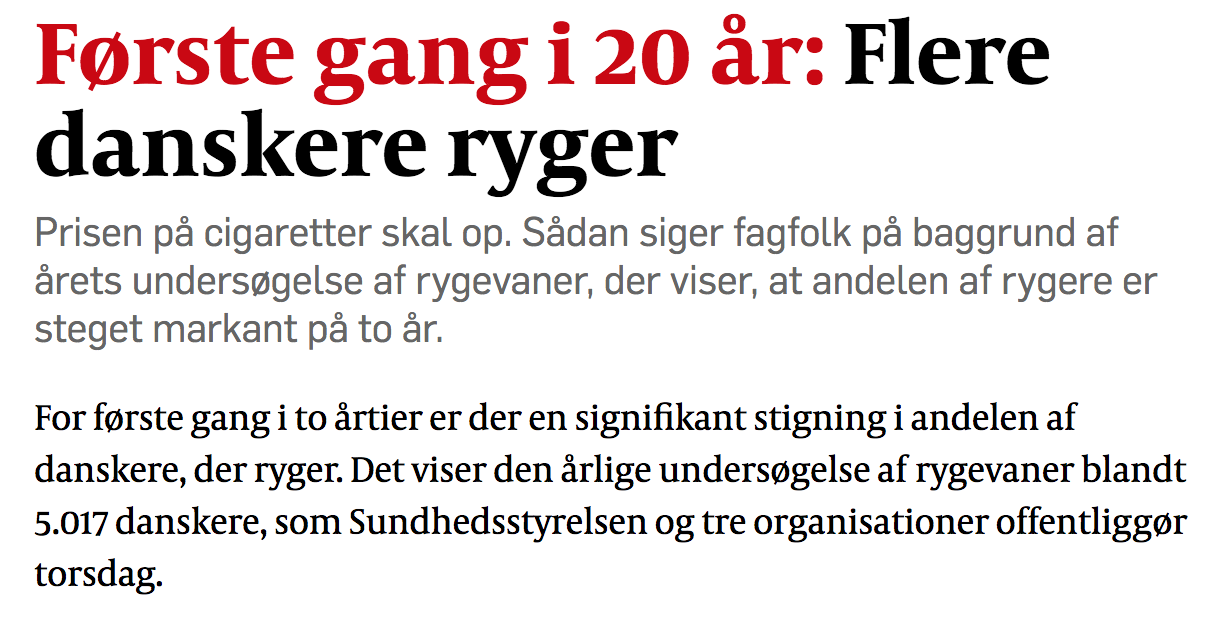
\includegraphics[scale=0.5]{rygere.png}
\end{frame}

\begin{frame}{Proportion of smokers in Denmark}
\center
\includegraphics[scale=0.5]{smokersData}
\end{frame}


\begin{frame}{Data analysis objectives}
  Focusing on the proportion of smokers in Denmark we wish to:
  \begin{enumerate}
    \item{Quantify the certainty by which the proportion of smokers is increasing in 2018.}
	\item{Find out when the proportion started to increase (if it is currently increasing).}
	\item{Assess if it is the first time in 20 years that the proportion has increased.}
  \end{enumerate}	  
\end{frame}

%\begin{frame}{Jyllands Posten February 19 2019}
%\center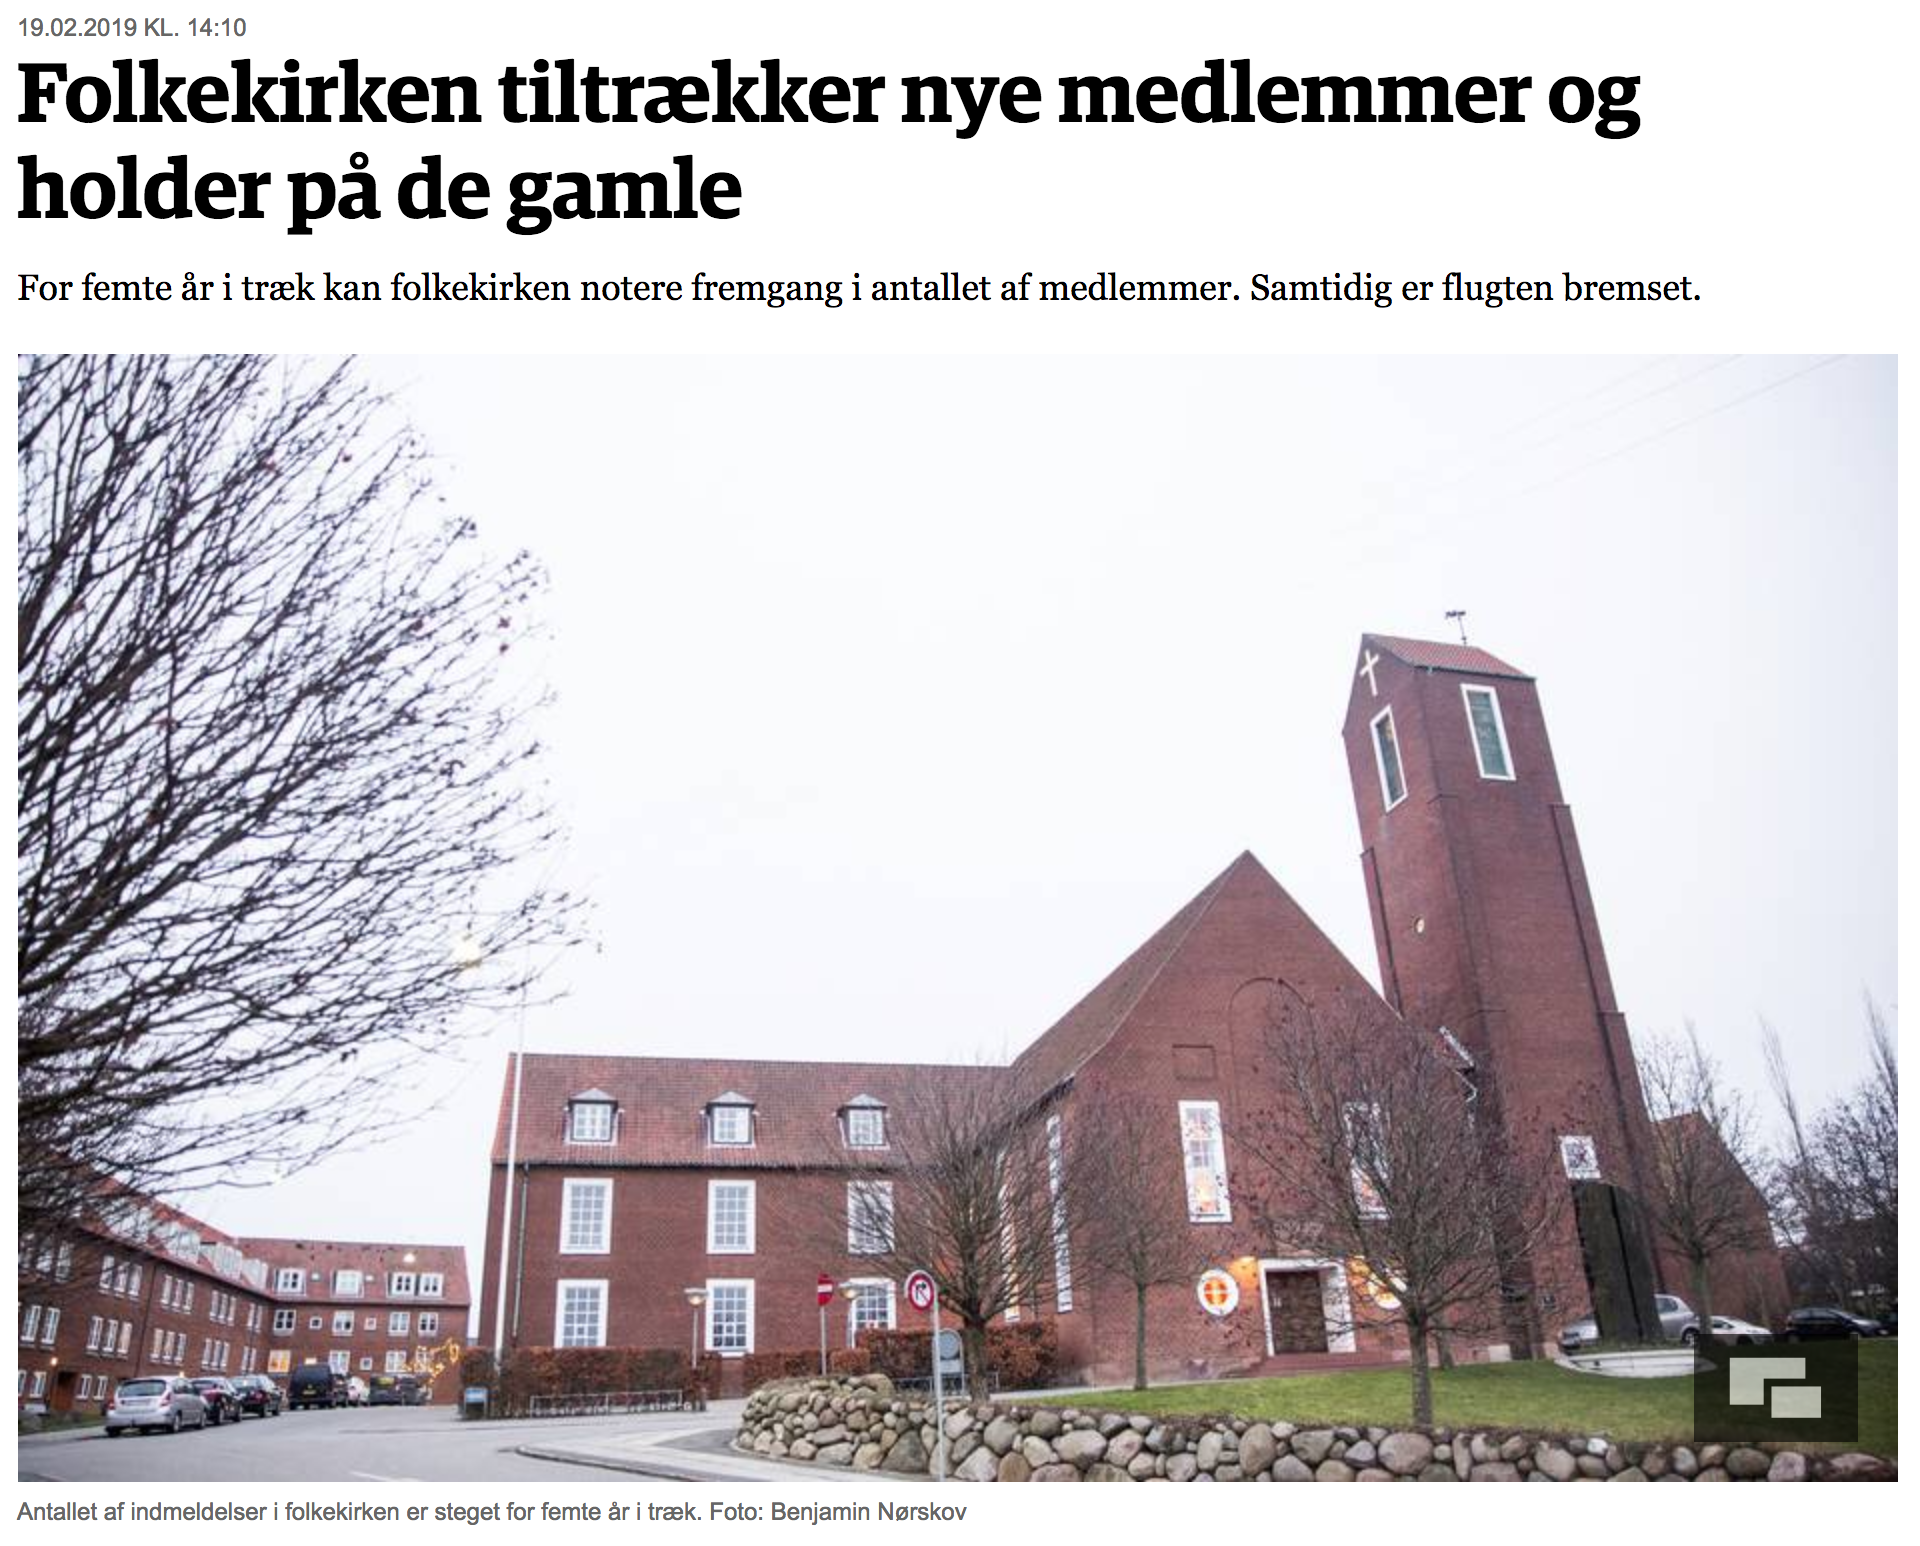
\includegraphics[scale=0.28]{baptisms.png}
%\end{frame}

\section{Six definitions}

\begin{frame}{Definition 1}
\begin{alertblock}{Definition 1}
  Reality evolves in continuous time $t \in \mathcal{T} \subset \mathbb{R}$.
\end{alertblock}  
\end{frame}


\begin{frame}{Definition 2}
\begin{alertblock}{Definition 2}
  There exists a latent function $f = \left\{f(t) : t \in \mathcal{T}\right\}$ governing the time evolution of some outcome. We observe random variables sampled from $f$ at discrete time points with additive measurement noise
  \begin{align*}
	  Y_i &= f(t_i) + \varepsilon_i, \quad t_i \in \mathcal{T}, \quad \E[\varepsilon_i \mid t_i] = 0
  \end{align*}
  
  We wish to understanding the dynamics of $f$ conditional on observed data $(Y_i, t_i)_{i=1}^{n}$.  
\end{alertblock}    
\end{frame}



\begin{frame}{Definition 3}
\begin{alertblock}{Definition 3}
  The \alert{trend} of $f$ is its instantaneous slope
  \begin{align*}
	  df(t) = \left(\frac{\mathrm{d} f(s)}{\mathrm{d}s}\right)(t)
  \end{align*}
  \begin{itemize}
    \item{$df(t) > 0$: $f$ is increasing at $t$ and has a \alert{positive trend}}
	\item{$df(t) < 0$: $f$ is decreasing at $t$ and has a \alert{negative trend}}
  \end{itemize}
\end{alertblock}    
\end{frame}



\begin{frame}{Definition 4}
\begin{alertblock}{Definition 4}
  A \alert{change in trend} of $f$ is when $df$ changes sign.
  \begin{itemize}
    \item{$f$ goes from increasing to decreasing or vice versa}
	\item{The trend, $df$, goes from positive to negative or vice versa}
  \end{itemize}
  
  \pause
 
  \vspace{1cm}
  
  A change in trend does not occur at a unique point in time. The question is:
  \begin{quotation}
	  ,,What is the \alert{probability} that the trend is changing at $t$ given everything we know?''
  \end{quotation}
\end{alertblock}    
\end{frame}


\begin{frame}{Definition 5}
\begin{alertblock}{Definition 5}
  The \alert{Trend Direction Index} (called Teddy) is the conditional probability
  \begin{align*}
    \mathrm{TDI}(t, \delta) = P(df(t + \delta) > 0 \mid \mathcal{F}_t)
  \end{align*}
  where $\mathcal{F}_t$ is the sigma algebra of all available information up until time $t$.
\end{alertblock}    

\pause

\vspace{0.5cm}
\begin{itemize}
	\item{TDI is a local probability.}
	\item{$\delta \leq 0$ is estimation. $\delta > 0$ is forecasting.}
	\item{Alternatively: $df(t + \delta) < 0$ but that is just $1 - \mathrm{TDI}(t, \delta)$.}
	\item{Common example: $t = \mathrm{now}$ and $\delta = 0$ (change-point models are impossible).}
\end{itemize}
\end{frame}


\begin{frame}{Definition 6}
\begin{alertblock}{Definition 6}
  The \alert{Expected Trend Instability} (called Eddy) on an interval $\mathcal{I}$ is
  \begin{align*}
    \mathrm{ETI}(\mathcal{I}) = \E[\#\left\{t \in \mathcal{I} : df(t) = 0\right\} \mid \mathcal{F}]
  \end{align*}
\end{alertblock}    
The value is equal to:
\begin{itemize}
  \item{The expected number of trend changes in $\mathcal{I}$}
  \item{The expected number of zero-crossings by $df$ in $\mathcal{I}$}
\end{itemize}
ETI is a global measure and the lower $\mathrm{ETI}$ is, the more stable the trend is on an interval.
\end{frame}

\section{A Functional Data Approach for Assessing the Trendiness of Trends}

\begin{frame}{Teddy and Eddy}
We wish to estimate Teddy and Eddy from data. This requires:
\begin{enumerate}
  \item{A probabilistic model linking observed data to the latent function $f$.}
  \item{The distribution of $df$ conditional on data (for Teddy).}
  \item{The joint conditional distribution of $(df, d^2\!f)$ (for Eddy).}
\end{enumerate}

\vspace{0.8cm}

Using latent \alert{Gaussian Processes} we can easily derive these and estimate them from data.

\end{frame}

\begin{frame}{Latent Gaussian Process model}
\begin{alertblock}{Gaussian Process}
A random function $\left\{f(t) : t \in \mathcal{T}\right\}$ is a Gaussian Process if and only if $(f(t_1), \ldots, f(t_n))$ is multivariate normal distributed for every $(t_1, \ldots, t_n) \subset \mathcal{T}$ with $n < \infty$. 

We write $f \sim \mathcal{GP}(\mu(\cdot), C(\cdot, \cdot))$ where $\mu\colon\, \mathcal{T} \mapsto \mathbb{R}$ and $C\colon\, \mathcal{T} \times \mathcal{T} \mapsto \mathbb{R}$ are the mean and covariance functions.
\end{alertblock}

\pause

\vspace{1cm}

We assume that the observed data is generated by the following hierarchical model:
\begin{align*}
  f \mid \beta, \theta &\sim \mathcal{GP}(\mu_\beta(\cdot), C_\theta(\cdot,\cdot))\\
  Y_i \mid f(t_i), \Theta, t_i &\overset{iid}{\sim} N(f(t_i), \sigma^2), \quad \Theta = (\beta, \theta, \sigma^2)
\end{align*}
\end{frame}



\begin{frame}{Joint distribution}
Let $\mathbf{Y}$ be the vector of observed data at time points $\mathbf{t}$ and $\mathbf{t}^\ast$ any finite subset of $\mathcal{T}$.

\vspace{1cm}

The model implies the following joint distribution:
{\scriptsize
\begin{align*}
  \begin{bmatrix}f(\mathbf{t}^\ast)\\ df(\mathbf{t}^\ast)\\ \mathbf{Y}\end{bmatrix} \mid \mathbf{t}, \Theta \sim N\left(\begin{bmatrix}\mu_\beta(\mathbf{t}^\ast)\\ d\mu_\beta(\mathbf{t}^\ast)\\ \mu_\beta(\mathbf{t})\end{bmatrix}, \begin{bmatrix}C_\theta(\mathbf{t}^\ast,\mathbf{t}^\ast) & \partial_2 C_\theta(\mathbf{t}^\ast, \mathbf{t}^\ast) & C_\theta(\mathbf{t}^\ast, \mathbf{t})\\ \partial_1 C_\theta(\mathbf{t}^\ast, \mathbf{t}^\ast) &  \partial_1 \partial_2 C_\theta(\mathbf{t}^\ast, \mathbf{t}^\ast) & \partial_1 C_\theta(\mathbf{t}^\ast, \mathbf{t})\\ C_\theta(\mathbf{t}, \mathbf{t}^\ast) & \partial_2 C_\theta(\mathbf{t}, \mathbf{t}^\ast) & C_\theta(\mathbf{t}, \mathbf{t}) + \sigma^2 I\end{bmatrix}\right)
\end{align*}
}%

\begin{itemize}
  \item{$\mathbf{t}^\ast$ can be any finite vector in continuous time}
  \item{Directly extendable to include $d^2\!f$ (required for ETI)}
  \item{(sample path regularity conditions are implicitly assumed)}
\end{itemize}
\end{frame}



\begin{frame}{Joint posterior distribution}
The joint posterior distribution of the latent functions is
\begin{align*}
\begin{bmatrix}f(\mathbf{t}^\ast)\\ df(\mathbf{t}^\ast) \end{bmatrix} \mid \mathbf{Y}, \mathbf{t}, \Theta &\sim
N\left(\begin{bmatrix}\mu_f(\mathbf{t}^\ast)\\ \mu_{df}(\mathbf{t}^\ast)\end{bmatrix}, \begin{bmatrix}\Sigma_{f,f}(\mathbf{t}^\ast, \mathbf{t}^\ast) & \Sigma_{f,df}(\mathbf{t}^\ast, \mathbf{t}^\ast)\\ \Sigma_{f,df}(\mathbf{t}^\ast, \mathbf{t}^\ast)^T & \Sigma_{df,df}(\mathbf{t}^\ast, \mathbf{t}^\ast)\end{bmatrix}\right)
\end{align*}

{\footnotesize
\begin{align*}
  \mu_f(\mathbf{t}^\ast) &= \mu_{\beta}(\mathbf{t}^\ast) + C_\theta(\mathbf{t}^\ast, \mathbf{t})\left[C_\theta(\mathbf{t}, \mathbf{t}) + \sigma^2 I\right]^{-1}\left(\mathbf{Y} - \mu_\beta(\mathbf{t})\right)\nonumber\\
  \mu_{df}(\mathbf{t}^\ast) &= d\mu_{\beta}(\mathbf{t}^\ast) + \partial_1 C_\theta(\mathbf{t}^\ast, \mathbf{t})\left[C_\theta(\mathbf{t}, \mathbf{t}) + \sigma^2 I\right]^{-1}\left(\mathbf{Y} - \mu_\beta(\mathbf{t})\right)\nonumber\\
  \Sigma_{f,f}(\mathbf{t}^\ast, \mathbf{t}^\ast) &= C_\theta(\mathbf{t}^\ast, \mathbf{t}^\ast) - C_\theta(\mathbf{t}^\ast, \mathbf{t})\left[C_\theta(\mathbf{t}, \mathbf{t}) + \sigma^2 I\right]^{-1} C_\theta(\mathbf{t}^\ast, \mathbf{t})^T\nonumber\\
  \Sigma_{df,df}(\mathbf{t}^\ast, \mathbf{t}^\ast) &= \partial_1 \partial_2 C_\theta(\mathbf{t}^\ast, \mathbf{t}^\ast) - \partial_1 C_\theta(\mathbf{t}^\ast, \mathbf{t})\left[C_\theta(\mathbf{t}, \mathbf{t}) + \sigma^2 I\right]^{-1} \partial_1 C_\theta(\mathbf{t}^\ast, \mathbf{t})^T\nonumber\\
  \Sigma_{f,df}(\mathbf{t}^\ast, \mathbf{t}^\ast) &= \partial_1 C_\theta(\mathbf{t}^\ast, \mathbf{t}^\ast) - C_\theta(\mathbf{t}^\ast, \mathbf{t})\left[C_\theta(\mathbf{t}, \mathbf{t}) + \sigma^2 I\right]^{-1}\partial_1 C_\theta(\mathbf{t}^\ast, \mathbf{t})^T\nonumber
\end{align*}
}%
\end{frame}

\begin{frame}{Trend Direction Index}
Recall the definition of the \alert{Trend Direction Index}
\begin{align*}
  \mathrm{TDI}(t, \delta) = P(df(t + \delta) > 0 \mid \mathcal{F}_t)	
\end{align*}

\vspace{0.8cm}

Letting $\mathcal{F}_t = \sigma\left\{\mathbf{Y}, \mathbf{t}\right\}$, we may express TDI through the posterior of $df$ as
\begin{align*}
  \mathrm{TDI}(t, \delta \mid \Theta) &= P\left(df(t + \delta) > 0 \mid \mathbf{Y}, \mathbf{t}, \Theta\right)\\
        &= \int_0^\infty N\left(u, \mu_{df}(t + \delta), \Sigma_{df,df}(t + \delta,t + \delta)^{1/2}\right)\mathrm{d}u
\end{align*}
\end{frame}


\begin{frame}{Example - prior distribution of $f$}
  What the world could look like with eyes closed
  \center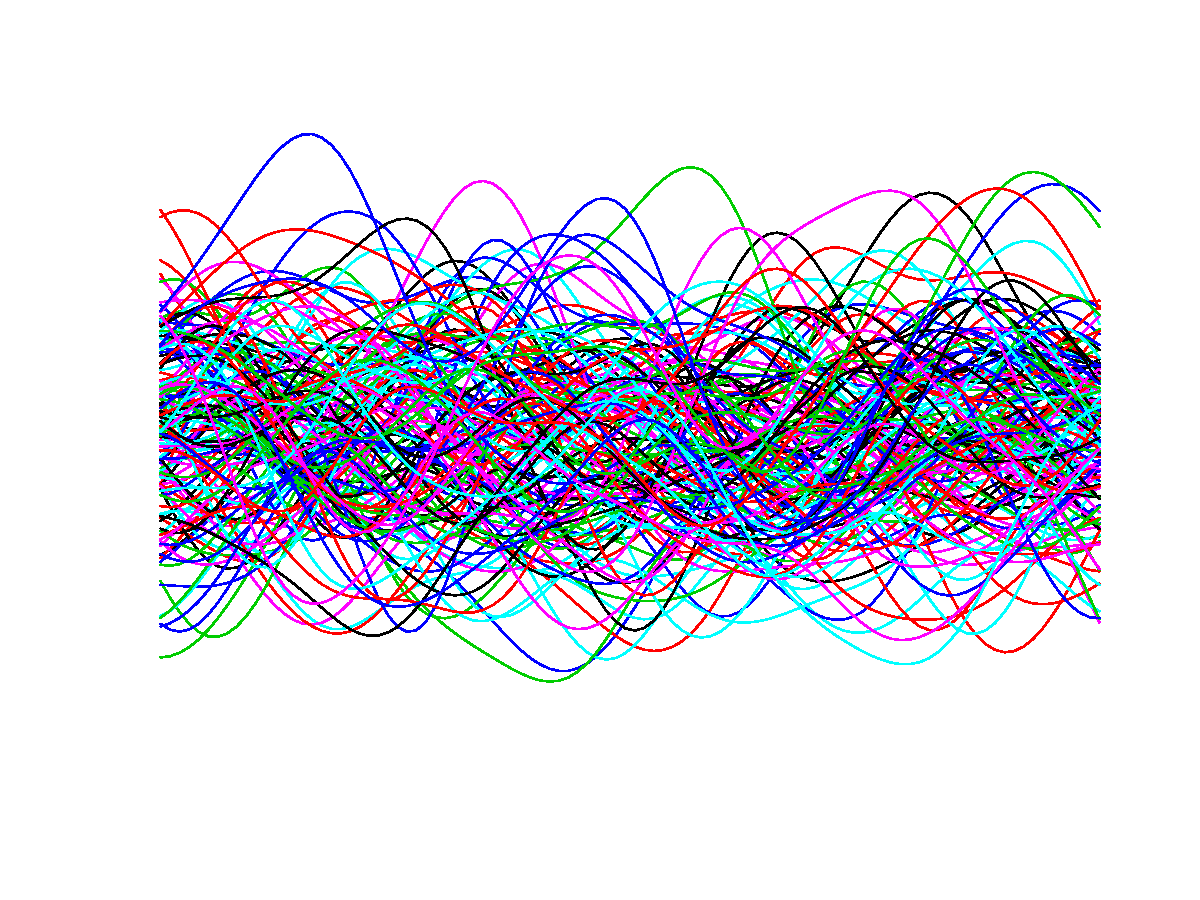
\includegraphics[scale=0.5]{postAni01}
\end{frame}

\begin{frame}{Example - posterior distribution of $f$ and TDI}
  \center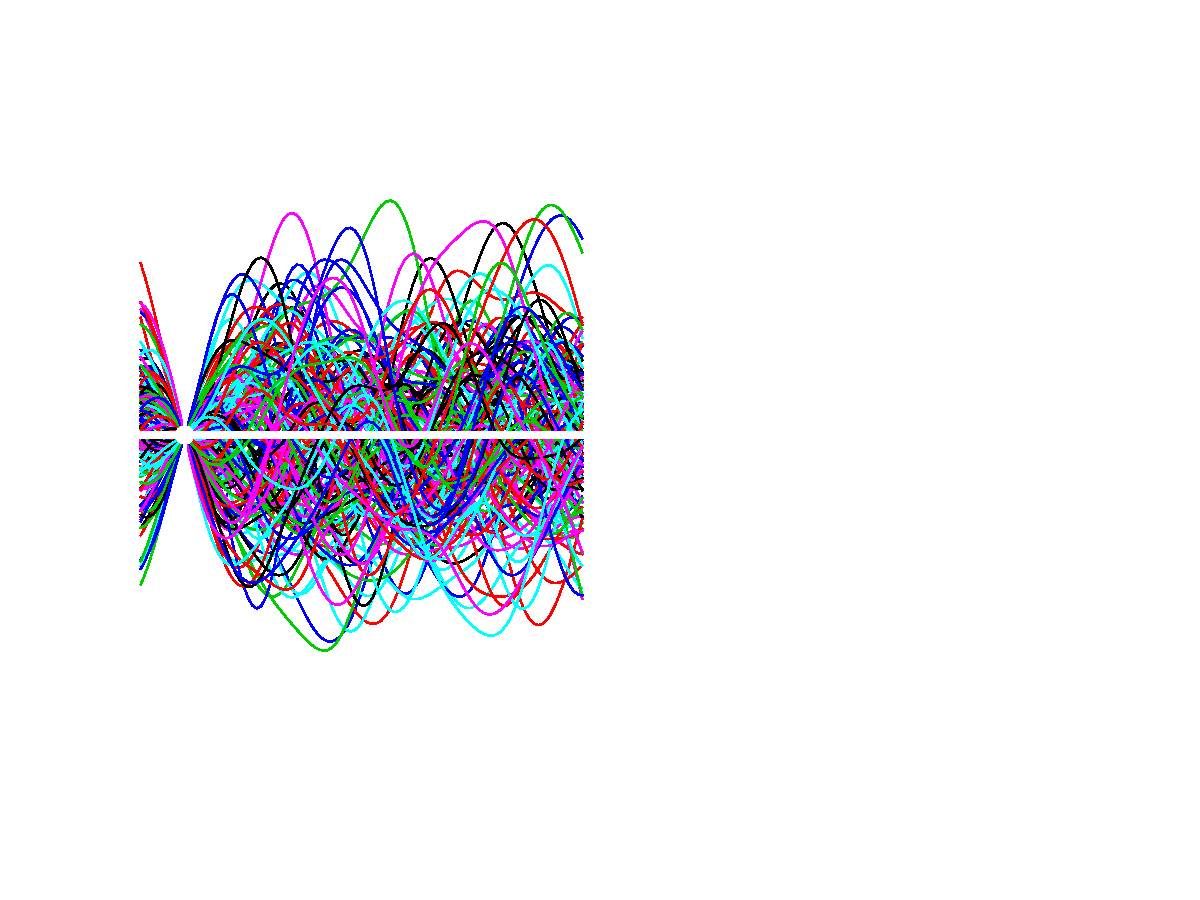
\includegraphics[scale=0.5]{probAni01}
\end{frame}

\begin{frame}{Example - posterior distribution of $f$ and TDI}
  \center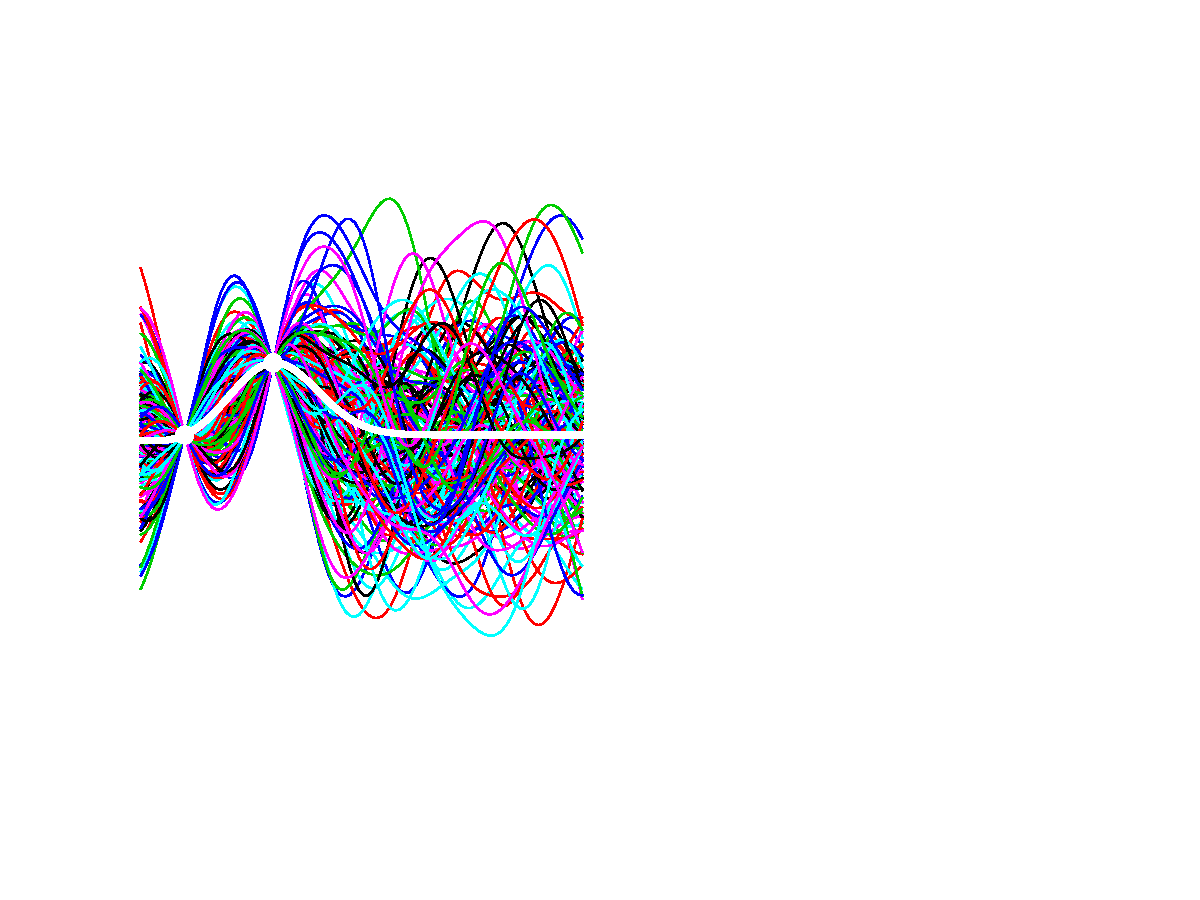
\includegraphics[scale=0.5]{probAni02}
\end{frame}

\begin{frame}{Example - posterior distribution of $f$ and TDI}
  \center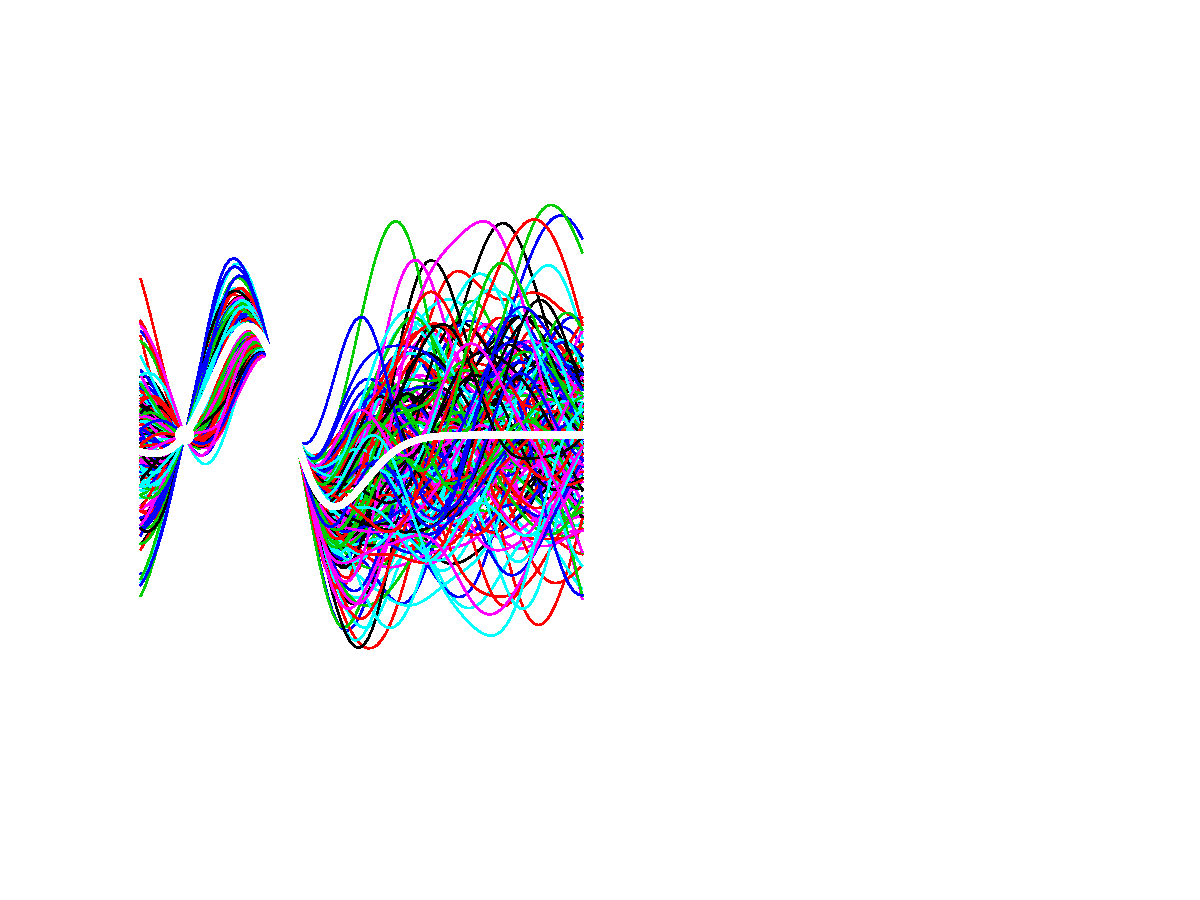
\includegraphics[scale=0.5]{probAni03}
\end{frame}

\begin{frame}{Example - posterior distribution of $f$ and TDI}
  \center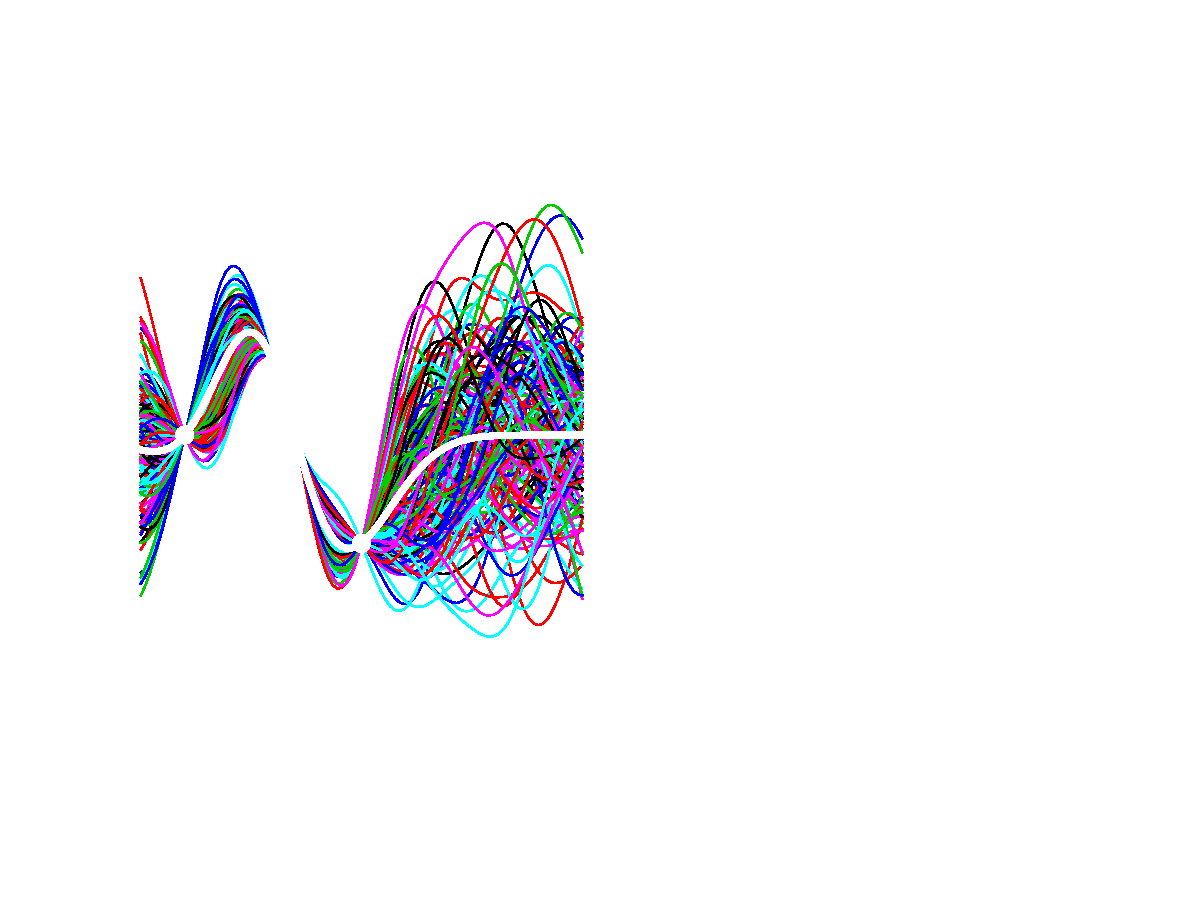
\includegraphics[scale=0.5]{probAni04}
\end{frame}

\begin{frame}{Example - posterior distribution of $f$ and TDI}
  \center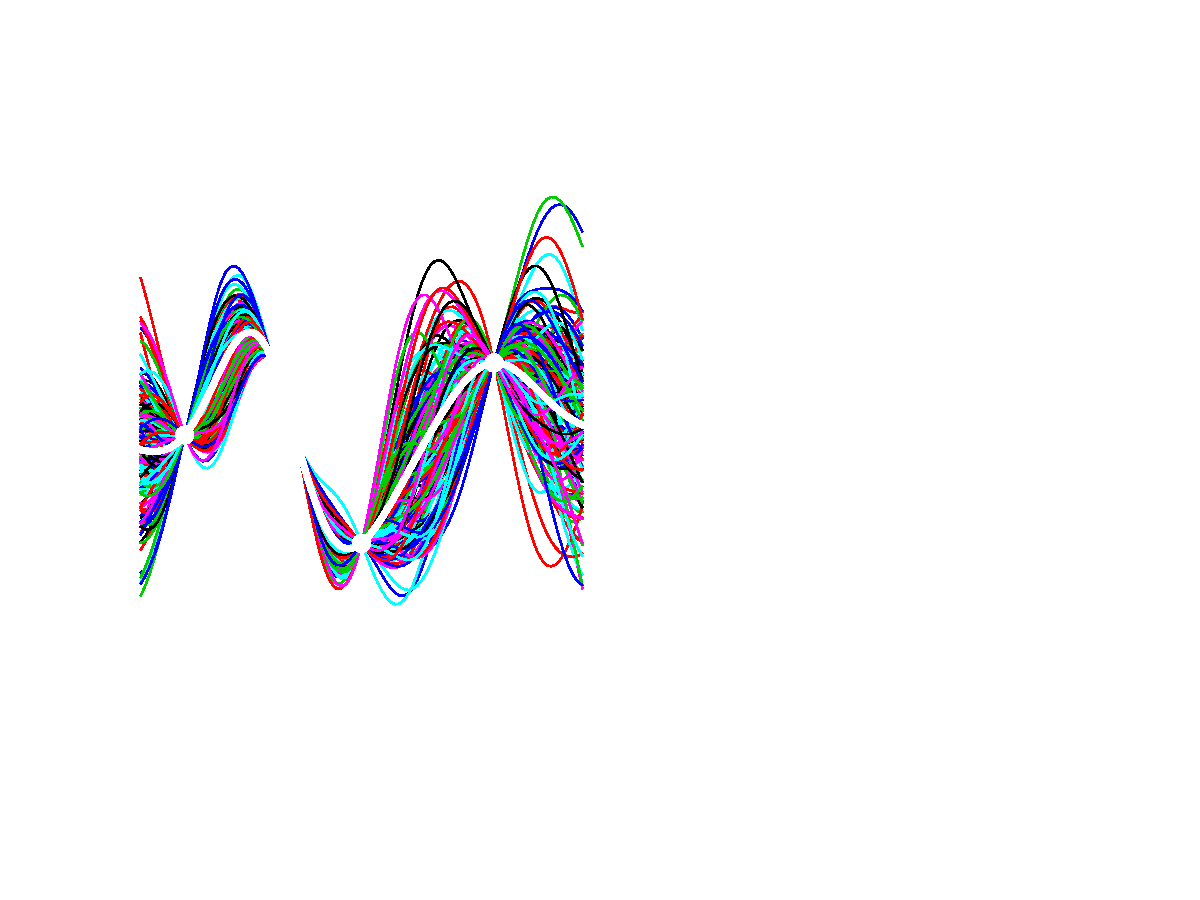
\includegraphics[scale=0.5]{probAni05}
\end{frame}

\begin{frame}{Example - posterior distribution of $f$ and TDI}
  \center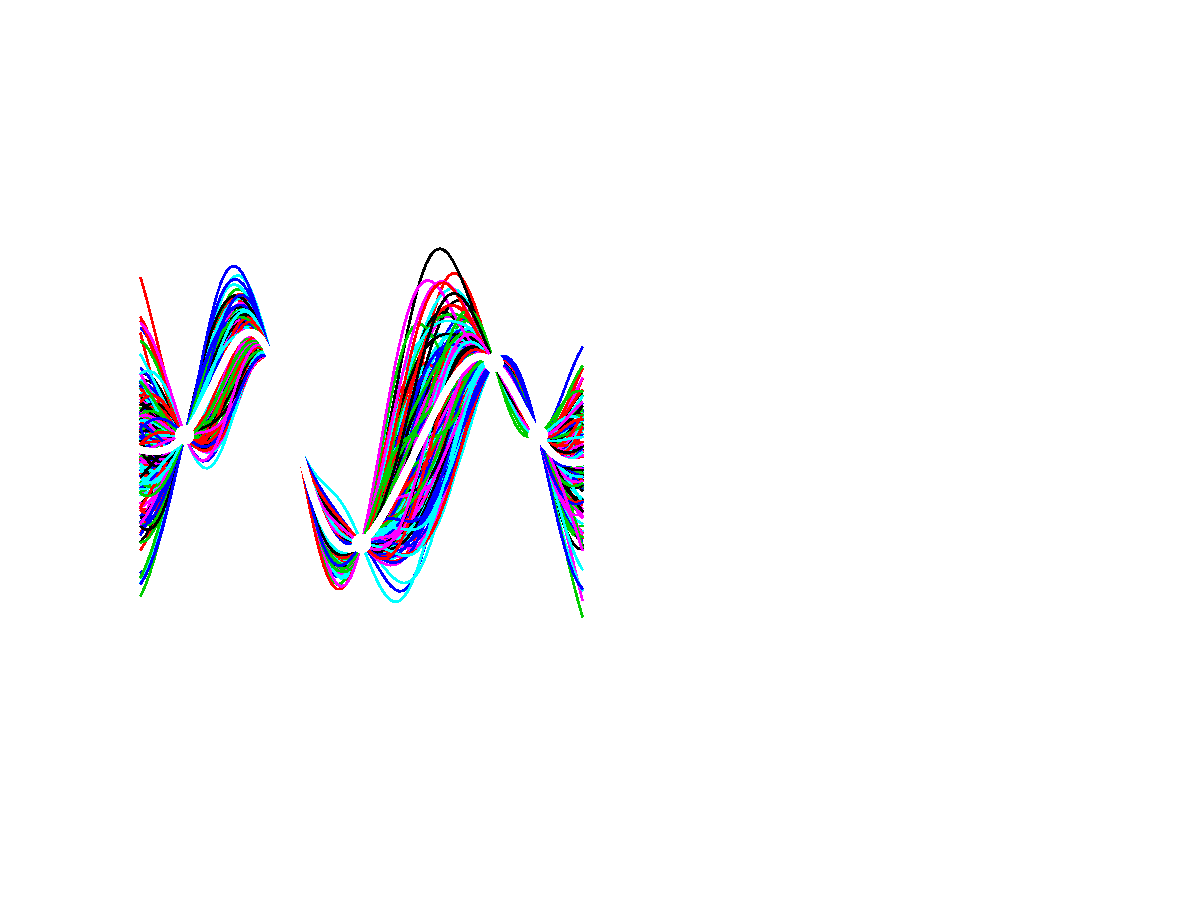
\includegraphics[scale=0.5]{probAni06}
\end{frame}

\begin{frame}{Expected Trend Instability}
  Recall the definition of the Expected Trend Instability
  \begin{align*}
    \mathrm{ETI}(\mathcal{I}) = \E[\#\left\{t \in \mathcal{I} : df(t) = 0\right\} \mid \mathcal{F}]
  \end{align*}
  Rice (1944) showed that the expected number of 0-crossings of a process $X$ under suitable regularity conditions is equal to
  \begin{align*}
    \mathrm{ETI}(\mathcal{I}) = \int_\mathcal{I}\int_{-\infty}^\infty |v| f_{X(t), dX(t)}(0, v)\mathrm{d}v\mathrm{d}t
  \end{align*}
  where the integrand is the \alert{local crossing intensity}. 
  
  \pause
  
  \vspace{0.5cm}
  We need to calculate this for the posterior distribution of $(df, d^2\!f)$. We obtain:
{\tiny
  \begin{align*}
    \mathrm{ETI}(\mathcal{I} \mid \Theta) = \int_{\mathcal{I}} \frac{\Sigma_{d^2\!f}(t,t)^{1/2}}{\Sigma_{df}(t,t)^{1/2}} \sqrt{1 - \omega(t)^2}   \phi\left(\frac{\mu_{df}(t)}{\Sigma_{df}(t,t)^{1/2}}\right)\left[2\phi(\zeta(t)) + \zeta(t) \Erf\left(\frac{\zeta(t)}{\sqrt{2}}\right)\right]\mathrm{d}t
  \end{align*}
  \begin{align*}
  \omega(t) = \frac{\Sigma_{df,d^2\!f}(t,t)}{\Sigma_{df}(t,t)^{1/2}\Sigma_{d^2\!f}(t,t)^{1/2}}, \quad \zeta(t) = \frac{\mu_{d^2\!f}(t) - \mu_{df}(t)\Sigma_{d^2\!f}(t,t)^{1/2}\omega(t)\Sigma_{df}(t,t)^{-1/2}}{\Sigma_{d^2\!f}(t,t)^{1/2}(1 - \omega(t)^2)^{1/2}}
  \end{align*}
}
\end{frame}


\begin{frame}{Example - Expected Trend Instability}
  \center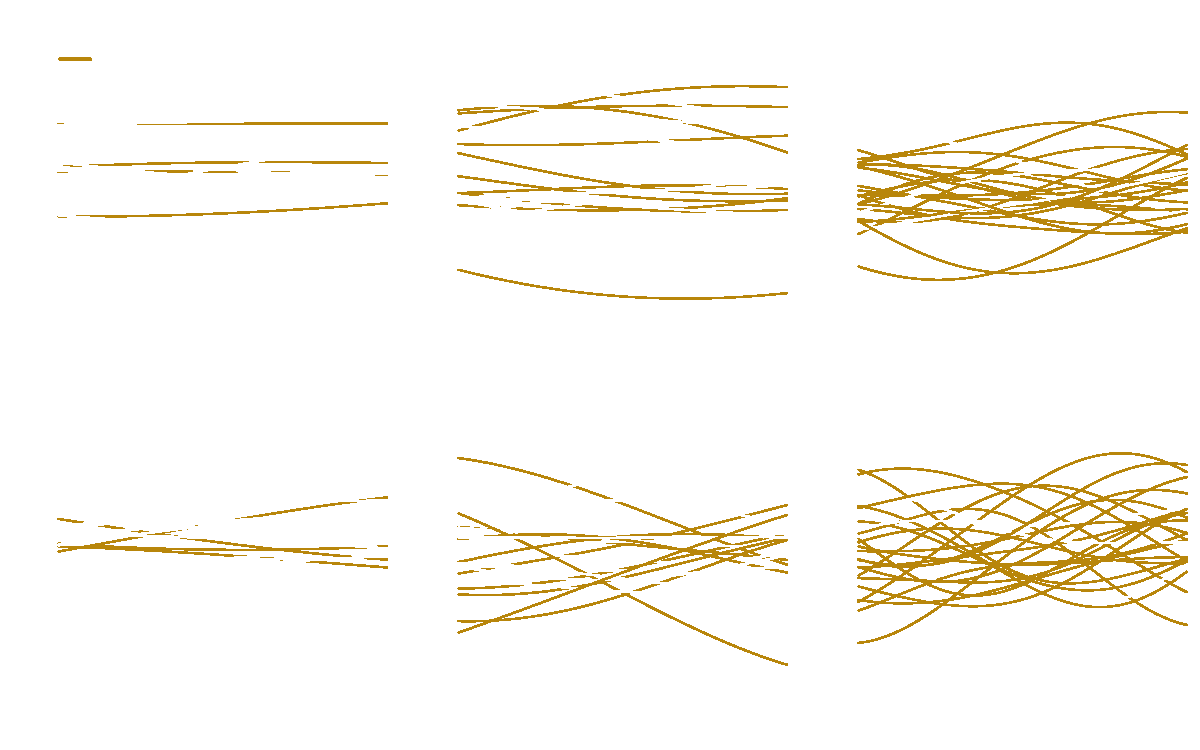
\includegraphics[scale=0.55]{ETIexample}
\end{frame}


\section{Estimation}
\begin{frame}{Maximum Marginal Likelihood}
The marginal likelihood is analytically available by integrating out the latent process
\begin{align*}
  L(\Theta \mid \mathbf{Y}, \mathbf{t}) = N(\mathbf{Y}; \mu_\beta(\mathbf{t}), C_\theta(\mathbf{t}, \mathbf{t}) + \sigma^2 I)
\end{align*}
leading to the estimate $\widehat{\Theta} = \argsup_{\Theta} L(\Theta \mid \mathbf{Y}, \mathbf{t})$.

\vspace{1cm}

\pause

This gives us the \alert{point estimates} of Eddy and Teddy:
\begin{align*}
  \text{TDI}(t, \delta \mid \widehat{\Theta}), \quad   \text{ETI}(\mathcal{T} \mid \widehat{\Theta})
\end{align*}


But it is difficult to obtain their distributions which are required in order to assess their uncertainties.
\end{frame}




\begin{frame}{Bayesian estimation}
Another approach is a fully Bayesian model with a prior distribution on the parameters of the latent function, $\Theta \sim G$.

This enables posterior distributions of $\text{TDI}(t, \delta \mid \Theta)$ and $\text{ETI}(\mathcal{T} \mid \Theta)$ using Markov-chain Monte Carlo simulation.

We have implemented the model in Stan.

\vspace{1cm}

\pause 

We use moderately informative priors for $\Theta$ centered at the marginal maximum likelihood estimates but with heavy tails and large variances.

We ran 4 chains for 25,000 iterations (half for warm-up).
\end{frame}



\section{Application}

\begin{frame}{From the Danish Health Authority\footnotemark}
\center
\includegraphics[scale=0.38]{rygereSST1.png}
%\center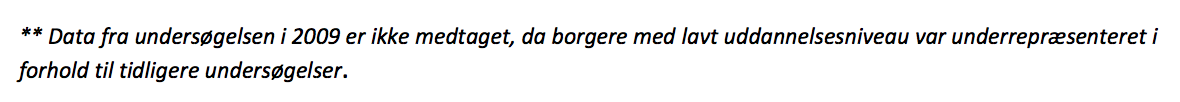
\includegraphics[scale=0.42]{rygereSST2.png}
\center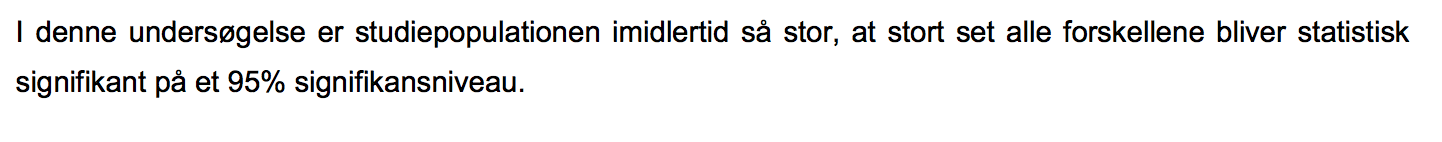
\includegraphics[scale=0.41]{rygereSST3.png}
\footnotetext[1]{\tiny Nøgletal - Danskernes rygevaner 2018, \texttt{www.sst.dk/da/udgivelser/2019/danskernes-rygevaner-2018}}
\end{frame}


\begin{frame}{Proportion of smokers in Denmark}
\center
\includegraphics[scale=0.5]{smokersData}
\end{frame}

\begin{frame}{Simple analysis - Has the proportion in 2018 changed?}
A simple analysis is to test whether the proportion of smokers in 2018 has changed compared to a previous year. Just a $\chi^2$-test.

\begin{table}
\center
\begin{tabular}{c|r|}
Comparison & p-value\\\hline
2018 vs. 2017 & 0.074\\
2018 vs. 2016 & \textbf{0.020}\\
2018 vs. 2015 & 0.495\\
2018 vs. 2014 & \textbf{0.012}\\
2018 vs. 2013 & 0.576\\
\end{tabular}
\end{table}

\vspace{0.5cm}

Conclusion?
\end{frame}

\begin{frame}{Simple analysis - It is the first time the trend has changed?}
A simple approach is to look at how often $1(Y(t_{i+1}) - Y_{t_i} > 0)$ jumps. 

9 jumps. Many of them are probably just noise.

\center
\includegraphics[scale=0.45]{jumpPlot}
\end{frame}


\begin{frame}{Trendiness analysis - Model selection}
Before fitting the model we need to select a prior mean and covariance function for the Gaussian Process. 

\vspace{0.6cm}

We consider 12 different models and compare them by Maximum Marginal Likelihood based LOO MSEP.

\begin{table}[htbp]
\center
\begin{tabular}{l|rrrr}
 & SE & RQ & Matern 3/2 & Matern 5/2\\ \hline
Constant & 0.682 & \textbf{0.651} & 0.687 & 0.660\\
Linear & 0.806 & $\Leftarrow	$ & 0.896 & 0.865\\
Quadratic & 0.736 & $\Leftarrow$ & 0.800 & 0.785
\end{tabular}
\end{table}

\begin{align*}
  \Theta_{-i}^\mathcal{M} &= \argsup_{\Theta} N\left(\mathbf{Y}_{-i}; \mu_\beta^\mathcal{M}(\mathbf{t}_{-i}), C_\theta^\mathcal{M}(\mathbf{t}_{-i}, \mathbf{t}_{-i}) + \sigma^2 I\right)\\
  \text{MSPE}_{\text{LOO}}^\mathcal{M} &= \frac{1}{n}\sum_{i=1}^{n} \left(Y_i - \E[f(t_i) \mid \mathbf{Y}_{-i}, \mathbf{t}_{-i} \Theta_{-i}^\mathcal{M}]\right)^2
\end{align*}
\end{frame}

\begin{frame}{Trendiness analysis - Maximum Likelihood fit}
\center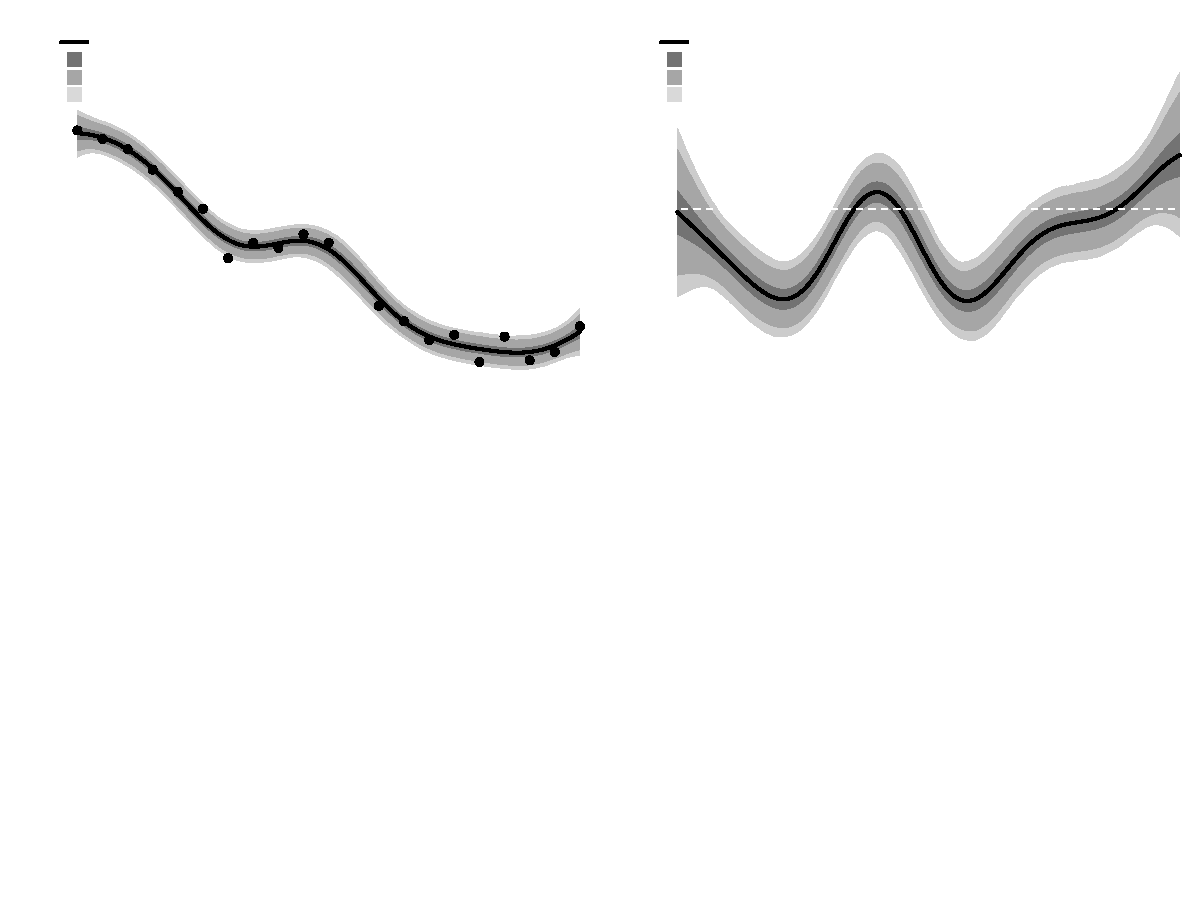
\includegraphics[scale=0.47]{fitLogLik}
\end{frame}

\begin{frame}{Trendiness analysis - Bayesian fit}
\center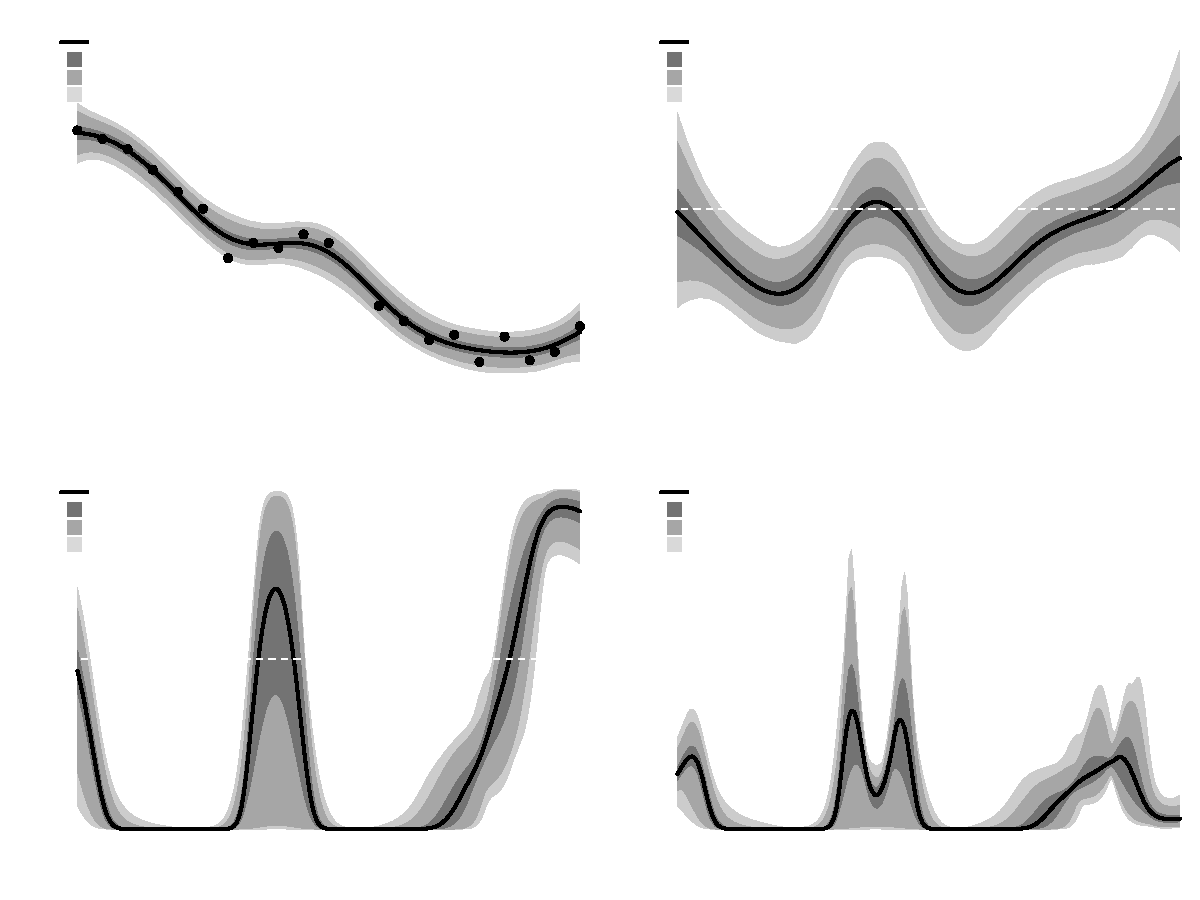
\includegraphics[scale=0.47]{fitBayes}	
\end{frame}

\begin{frame}{Trendiness analysis - Posterior ETI}
\center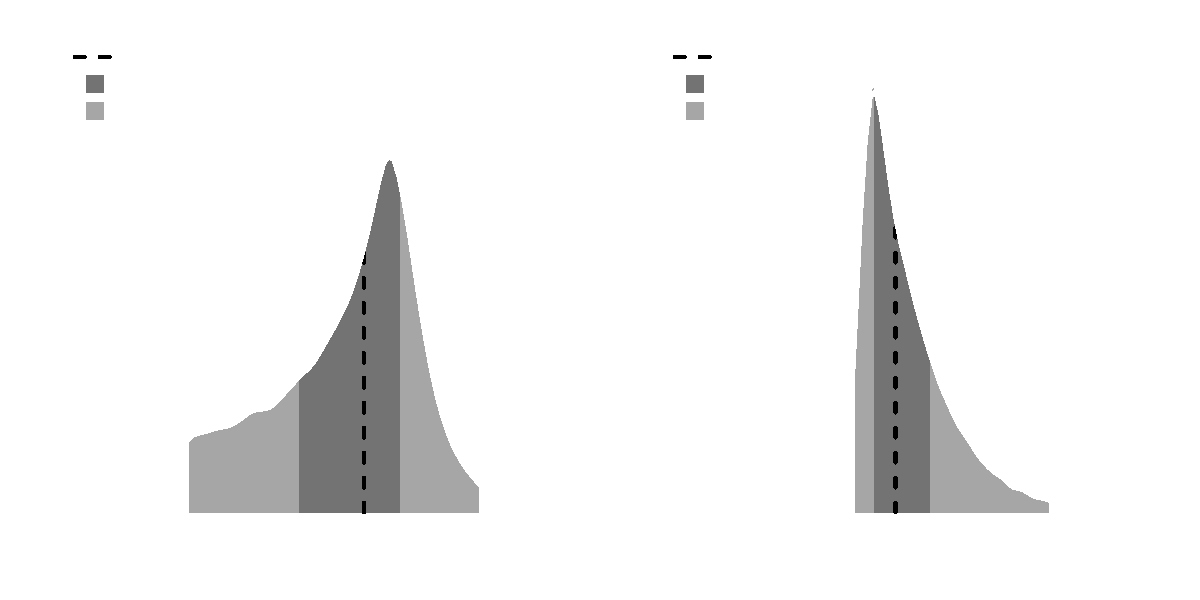
\includegraphics[scale=0.5]{ETIplot}	
\end{frame}


\begin{frame}{Conclusions}
Maximum Marginal Likelihood analysis:
{\footnotesize
\begin{itemize}
  \item{TDI(2018) = 95.24\%}
  \item{ETI([1998; 2018]) = 3.68}
  \item{ETI([2008; 2018]) = 1.39}
\end{itemize}
}

Bayesian analysis:
{\footnotesize
\begin{itemize}
  \item{Mean TDI in 2018 = 93.37\% (95\% CI = [82.22\%; 98.87\%])}
  \item{Median ETI([1998; 2018]) = 3.36 (95\% CI = [1.22; 4.76])}
  \item{Median ETI([2008; 2018]) = 1.26 (95\% CI = [1.02; 2.20])}
\end{itemize}
}

\pause

\alert{Conclusions:}
{\footnotesize
\begin{itemize}
  \item{We are currently (positively) trending with a very high probability.}
  \item{We have been trending with probability $> 50\%$ since sometime between 2015 and 2016.}
  \item{The expected number of changes in trend during the last 20 years is higher than stipulated.}
\end{itemize}
}
\end{frame}

\begin{frame}{Summary}
We have tried to answer the questions:
\begin{enumerate}
  \item{What is the probability of having positive trend at a given time?}
  \item{What is the expected number of times that a trend has changed on an interval?}
\end{enumerate}

Functional Data Analysis using latent Gaussian Processes is a flexible way to obtain such answers.
\end{frame}




\begin{frame}
\center \Huge Thank you!
\end{frame}


\end{document}

